\section{Ejercicio 6: Dise\~no e implementaci\'on de multivibradores biestables}
Basándose en compuertas lógicas discretas, se pretende diseñar, implementar y caracterizar circuitos que se comporten como multivibradores biestables de tipo Latch SR y 
Flip-Flop D.
Con la intensión de proveer parámetros de comparación que contextualicen a los diseños logrados, serán también medidos circuitos equivalentes comerciales, los cuales vienen 
ya integrados en un solo componente. \\
Las magnitudes que se consideran de interés para la caracterización de los diseños son los tiempos de propagación, rise, fall, set up y hold, así como cualquier otro 
fenómeno que resulte particularmente interesante al ser observadas las respuestas de los circuitos ante sus estímulos.



\subsection{Diseño de los circuitos}
Se presenta a continuación el desarrollo teórico necesario para el diseño de cada uno de los circuitos a partir de compuertas lógicas discretas.


\subsubsection{Latch SR}
El componente conocido como Latch SR es aquel que cumple con la tabla de verdad expresada en \ref{table:latch_sr_truth_table_ex6}.
Esta tabla de verdad puede ser implementada mediante el circuito presentado en la figura \ref{fig:latch_sr_with_gates_ex6}.

\begin{table}[H]
    \centering
    \begin{tabular}{cc|cc|c}
    \textbf{S} & \textbf{R} & \textbf{Q} & \textbf{~Q} & \textbf{Validez del estado} \\ \hline
    0          & 0          & Q          & ~Q          & \multirow{3}{*}{Válidos}    \\
    0          & 1          & 0          & 1           &                             \\
    1          & 0          & 1          & 0           &                             \\ \cline{5-5} 
    1          & 1          & 0          & 0           & Inválido                   
    \end{tabular}
    \caption{Tabla de verdad del Latch SR.}
    \label{table:latch_sr_truth_table_ex6}
\end{table}

\begin{figure}[H]
    \centering
    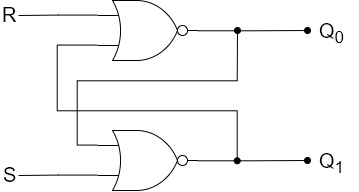
\includegraphics[width=0.8\textwidth]{../EJ6/Recursos/latch_sr_with_gates}
    \caption{Circuito Latch SR con compuertas lógicas discretas.}
    \label{fig:latch_sr_with_gates_ex6}
\end{figure}


\subsubsection{Flip-Flop D}
La tabla de verdad que representa a un Flip-Flop D es, por el contrario, la de la tabla \ref{table:ffd_truth_table_ex6}.
Luego, el circuito de implementación es el de la figura \ref{fig:ffd_with_gates_ex6}.
La parte del circuito indicada como Edge detector cumple la función de ser un detector de flancos que habilitará al circuito unicamente durante el tiempo que lo permite 
el retardo de las compuertas NOT no ideales que lo conforman.

\begin{table}[H]
    \centering
    \begin{tabular}{cc|cc}
    \textbf{S}   & \textbf{R} & \textbf{Q} & \textbf{~Q} \\ \hline
    $\uparrow$   & 0          & 0          & 1           \\
    $\uparrow$   & 1          & 1          & 0           \\
    X            & X          & Q          & ~Q         
    \end{tabular}
    \caption{Tabla de verdad del Flip-Flp D.}
    \label{table:ffd_truth_table_ex6}
\end{table}

\begin{figure}[H]
    \centering
    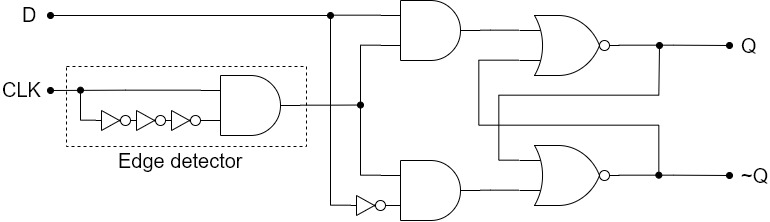
\includegraphics[width=0.8\textwidth]{../EJ6/Recursos/ffd_with_gates}
    \caption{Circuito Flip-Flop D con compuertas lógicas discretas.}
    \label{fig:ffd_with_gates_ex6}
\end{figure}



\subsection{Implementación en PCB}
